\documentclass[runningheads]{llncs}
\usepackage[T1]{fontenc}
\usepackage{graphicx}
\usepackage{subcaption}

\usepackage[commandnameprefix=always, defaultcolor=red]{changes}  %使用changes宏包
% \usepackage[final]{changes} %禁用修订,输出最终修订完成的版本
\definechangesauthor[name={zheliku}, color=blue]{zheliku} %修订作者

\bibliographystyle{splncs04}

\AtBeginDocument{%
  \providecommand\BibTeX{{%
    Bib\TeX}}}

\begin{document}

\title{VRTI: Providing Realistic Haptic Feedback and Hand Manipulation for Immersive Physics Learning}

% \author{Hailin Ji\inst{1} \and 
% % \orcidID{0009-0002-3512-6730} 
% Yihang Li\inst{1} \and 
% Yiran Zhang\inst{1} \and 
% Hongwen Zhang\inst{1} \and 
% Xiaoyan Hu\inst{1} \and 
% Yanhong Luo\inst{2}}
 
% \authorrunning{H. Ji et al.}

% \institute{Beijing Normal University, Beijing, China \and
% Northwest Minzu University, Beijing, China}

\author{Anonymous Author(s)}

\maketitle

\begin{abstract}
As gesture tracking technology matures, VR-based immersive learning environments enable Gesture Interaction (GI) with virtual objects, offering intuitive educational experiences. However, the absence of haptic feedback in GI compromises immersion. 
\chadded[id=zheliku]{
  This paper proposes Virtual-Real Twin Interaction (VRTI), which synchronizes Virtual Interactive Objects (VIO) with Real Interactive Objects (RIO) to provide dynamic haptic feedback for gestures. Key innovations include: 
  1) \textbf{Dynamization of static haptics}: Real-time sensor networks transform physical props' static properties into dynamic feedback through spatiotemporal synchronization. 
  2) \textbf{Gesture-prop consistency model}: Achieves visuo-haptic synchronized interaction, and supports interaction calibration during hand manipulations.
  Applied to high school momentum conservation experiments, three VR twins (puller/button/knob) support grasping, pressing, and pinching. Controlled trials (VRTI: N=32 vs GI: N=32) demonstrate that VRTI: 1) Significantly enhanced motivation (p<0.001) and immersion (p<0.001). 2) Reduced extraneous cognitive load (p<0.001, |r|=0.625). 3) higher experimental understanding (p=0.05) and better comprehension application (p=0.005)
}

\keywords{Virtual-Real Twin Interaction \and Virtual Reality \and Haptic Feedback \and Physics Prop \and Immersive Physics Learning \and Gesture Interaction}
\end{abstract}

\section{INTRODUCTION}
With the rapid advancement of VR technology, immersive learning environments have become a focal point of research and are widely applied in fields such as entertainment, education, and healthcare \cite{luo2020dream,yeung2021virtual}. Introducing immersive learning environments into physics experiment teaching can address the challenges faced by traditional methods, such as difficulties in understanding, high costs, cumbersome operations, and limited resources \cite{yang2007impact,abu2018design}. By transforming traditional teaching models, immersive learning environments create more interactive and engaging experiences, thereby stimulating students' interest and motivation. For instance, studies by Dalgarno \& Lee demonstrate that immersive learning environments significantly enhance students' ability to understand complex concepts and promote deep learning \cite{dalgarno2010learning}. Similarly, Campos et al. utilized immersive learning environments in introductory physics courses to teach vector concepts, allowing students to manipulate vectors in a 3D grid, identify their angular components, and measure their magnitudes. The results highlight the potential of this approach in fostering abstract conceptualization and operational skills, providing more intuitive explanations of physics concepts \cite{campos2022impact}.

Immersive learning environments offer new possibilities for physics experiment teaching by simulating experimental phenomena through visual and auditory means, reducing equipment requirements, and increasing experimental flexibility. However, the predominantly visual interaction lacks the haptic feedback present in real physical experiments, making it difficult for traditional immersive learning environments to provide an authentic physical operation experience \cite{giri2021application}. Learners in virtual environments can only observe physical phenomena but cannot feel the actual touch at play through haptic feedback, resulting in an incomplete learning experience. Physics experiments are not merely about observing phenomena but also involve direct perception of the interactions between forces and objects. Therefore, integrating haptic feedback into immersive physics learning environments is crucial. By incorporating haptic feedback, students can perceive the weight, resistance, and elasticity of objects in virtual environments, gaining a more intuitive operational experience and deepening their understanding of physics concepts and laws \cite{minaker2016handson}. Nevertheless, traditional haptic devices often provide only basic force feedback and may constrain learners' interactive actions, making it challenging to meet the demands of complex hand operations in physics experiments \cite{bonfert2023challenges}. For example, in real physics experiments, hand operations encompass a variety of actions, including grasping, pressing, pinching, rotating, and dragging. These operations not only require precise control of hand movements but also demand perception and adjustment of force magnitude, direction, and application, which are critical to the success of the experiment. However, existing haptic devices cannot accurately simulate these hand operations, resulting in a significant disparity between virtual experimentation and real-world operational fidelity.

In summary, this study makes the following key contributions.

First, we propose Virtual-Real Twin Interaction (VRTI), which integrates hand tracking with realistic haptic feedback into VR physics learning environments. The VRTI system comprises Virtual-Real twins (VR twins): a Virtual Interactive Object (VIO) for visual feedback and a Real Interactive Object (RIO) for haptic feedback. The RIO is fabricated using 3D printing technology based on 3D modeling designs, while the VIO is rendered in the virtual environment. Users directly manipulate these VR twins with both hands, achieving real-time synchronized visual and haptic feedback that delivers a highly realistic and natural interaction experience. This approach is characterized by high immersion, realistic haptic feedback, natural interaction, and low cost.

Second, we introduce a virtual-real alignment method for VRTI to avoid penetration issues between hands and VR twins. Position and orientation errors in hand tracking often cause penetration issues between the virtual hand and VIO. Our method addresses this visuo-haptic misalignment through gesture prediction optimization, eliminating penetration while maintaining interaction fidelity.

Finally, we validate the advantages of VRTI through an educational experiment. Collaborating with physics professors and researchers at XXX
% Beijing Normal 
University, we designed a momentum conservation experiment aligned with high school physics curricula. A controlled comparison between VRTI ($N=32$) and GI ($N=32$) demonstrates that VRTI:

\begin{itemize}
  \item Does not significantly increase cognitive load ($p = 0.602$);

  \item Significantly enhances learning motivation ($p < 0.001$) and immersion ($p < 0.001$);

  \item Improves comprehension of experimental content ($p = 0.05$) and knowledge application capabilities ($p = 0.005$) more effectively than GI alone.
\end{itemize}
\section{RELATED WORK}
\subsection{VR Learning Theories}
Research indicates that applying immersive VR in educational contexts can enhance students' learning experiences and improve their understanding of knowledge content \cite{freina2015literature}. Additionally, understanding and applying VR learning theories can help educators and researchers create better learning materials and assessment tools, as well as develop more effective teaching methods \cite{matovu2023immersive}. Therefore, the application of learning theories in the effective design of VR learning experiences has become increasingly important \cite{marougkas2023virtual}. Common VR learning theories include Cognitive Load Theory, the ARCS Model of Motivation, and Immersion Theory.

Cognitive Load Theory was proposed by John Sweller in 1988 as a framework for understanding learning and cognition \cite{sweller1988cognitive}. The theory posits that cognitive load can be categorized into three types: intrinsic, extraneous, and germane. Intrinsic cognitive load is related to the inherent complexity of the learning material and is unavoidable, depending on the task's complexity and the learner's prior knowledge. Extraneous cognitive load arises from unnecessary elements in instructional design that do not contribute to learning objectives. Germane cognitive load is associated with the construction and automation of cognitive structures during learning, which facilitate understanding and retention. A common perspective is that breaking down complex tasks into smaller components can reduce intrinsic cognitive load; eliminating unnecessary information and distractions can minimize extraneous cognitive load; and practice and repetition can increase germane cognitive load by helping learners build and automate schemas \cite{baceviciute2022investigating}.

The ARCS Model of Motivation, proposed by John M. Keller in 1987, is a widely used motivational framework in education \cite{keller1987development}. The model suggests that the stimulation and maintenance of learning motivation depend on four core elements: Attention, Relevance, Confidence, and Satisfaction. By capturing learners' interest (Attention), ensuring the relevance of learning content (Relevance), boosting learners' confidence (Confidence), and providing a sense of achievement (Satisfaction), the ARCS model helps educators design more engaging and effective instructional strategies. This model is not only applicable to traditional classrooms but is also widely used in modern educational technologies, such as VR education, serving as an important theoretical tool for enhancing learning motivation.

Immersion refers to the sense of being physically present in a virtual environment during user interaction. Sherman et al. categorize immersion into physical/sensory immersion and mental immersion \cite{sherman2003understanding}. In virtual environments, users gather information through senses such as vision, hearing, and touch, processed by their perceptual systems to enable free navigation and manipulation of virtual objects, achieving physical immersion. Mental immersion refers to a state of deep engagement in the virtual environment. Both types of immersion significantly impact user experience. Features such as free navigation, first-person perspectives, realism, and interactivity contribute to learners' sense of immersion \cite{regenbrecht2002real,mikropoulos2006presence}, with interactivity being particularly influential \cite{schubert2001experience}.

In addition to the above VR learning theories, new theoretical perspectives have recently gained attention among researchers. Ryan R M et al. proposed the Self-Determination Theory (SDT), emphasizing autonomy, competence, and relatedness in the learning process. VR technology, by providing immersive and interactive learning environments, better satisfies these psychological needs, thereby enhancing students' motivation and learning outcomes \cite{ryan2024self}. Liu J et al. explored how the autonomy of VR learning environments and learner characteristics jointly influence learning outcomes and cognitive load. Their results suggest that changes in a single factor do not necessarily alter outcomes, as they are often determined by the interaction of both factors \cite{liu2024autonomy}. Lui A L C et al. reviewed recent studies on VR education using learning theories and proposed six design principles to facilitate the transition from traditional classroom education to VR, offering theoretically grounded recommendations for future educators \cite{lui2023theory}.As technology advances and educational needs evolve, VR learning theories and practices will continue to develop and improve.

\subsection{Immersive Physics Learning}
With the advancement of VR technology, its application in immersive physics learning has become increasingly widespread. For example, Georgiou et al. introduced immersive VR into the theoretical learning of special relativity, allowing students to experience and explore related physical phenomena from a first-person perspective, thereby enhancing learning efficiency and motivation \cite{georgiou2021learning}. Campos et al. utilized immersive learning environments in introductory physics courses to teach vector concepts, enabling students to manipulate vectors in a 3D grid, identify their components and angles, and measure their lengths. This approach fosters the potential for abstract conceptualization and operational skills, providing more intuitive explanations of physics concepts and their relationship to the physical world \cite{campos2022impact}. Additionally, AR technology enhances user experiences by overlaying virtual objects onto real environments, making experimental elements that are typically unobservable visible and aiding students in deeply understanding scientific principles and content \cite{pegrum2021augmented,prahani2022trend}. For instance, many researchers have visualized force vectors in mechanics and electric potential distributions in electromagnetism in 3D, promoting students' understanding and cognition of complex physical phenomena \cite{al2020effectiveness,teichrew2020augmented,ismail2019enhancing,boettcher2021using}.

Despite the growing attention and discussion surrounding immersive physics learning environments, most research and practices still focus on using visual feedback to convey information, neglecting other sensory interactions. As a direct connection between the human body and the physical world, touch provides immediate information about shape, texture, temperature, and weight, playing an important role in human perceptual experiences\cite{zhang2023active}. Existing research shows that incorporating haptic feedback can significantly enhance the effectiveness of virtual learning environments. For example, Shen Yang et al. introduced haptic feedback technology into the design of K-12 physics experiment scenario, evaluating its application in immersive learning through quasi-experiments. The results indicate that using haptic feedback in VR immersive learning significantly improves learners' sense of realism and interaction efficiency, although it does not significantly impact knowledge gains \cite{shen2023research}. Johnson-Glenberg et al. demonstrated that in STEM education within virtual reality environments, adding haptic information significantly reduces cognitive load and enhances students' understanding and retention of knowledge, particularly when students have prior knowledge \cite{johnson2023embodied}. Furthermore, embodied cognition theory in education suggests that through physical perception and manipulation, learners can transform concrete experiences into abstract knowledge, reconstructing and simulating actual experiences at a psychological level \cite{varela2017embodied}. Haptic technology, by simulating real-world interactions, makes virtual experiments more engaging and realistic, effectively improving learning efficiency and playing an indispensable role in helping students understand complex concepts \cite{shapiro2019embodied}. Therefore, integrating haptic interaction into immersive physics learning environments and exploring optimal application models for haptics in immersive physics learning should become a future research trend and focus.

Currently, immersive physics learning environments supporting haptic feedback can be broadly categorized into two types: haptic feedback devices and AR-based systems. Hpatic feedback devices generate controllable physical forces through motors, hydraulic systems, or pneumatic systems, acting on the user's hands or body to simulate real-world haptic feedback. These forces can include tension, thrust, resistance, etc., providing a controlled haptic experience. Common haptic feedback devices in immersive physics learning environments include haptic feedback joysticks/robotic arms (e.g., PHANTOM series), haptic gloves (e.g., HaptX gloves), and vibration-based devices (e.g., VR controllers). For example, Qi K et al. designed an experimental interaction environment with liquid containers, using the Novint Falcon haptic feedback device to explore the impact of haptic and visual feedback on understanding fundamental physics concepts related to buoyancy \cite{qi2020impact}. Acevedo P et al. created a visualization environment for electromagnetism, using Oculus Quest VR controllers to provide vibration feedback and study the effects of virtual reality environments and haptic feedback on students' perception and understanding of electromagnetism \cite{acevedo2022effects}. On the other hand, AR technology overlays virtual information onto the real world, providing immersive haptic feedback through touchable physical objects (e.g., simulated tools or models). For instance, Knierim P et al. used tangible replicas to replace physical components in laboratory experiments, providing haptic feedback and visualizing workflows through AR. They compared users' performance in setup time, experienced workload, measurement quality, and conceptual understanding of learning tasks \cite{knierim2020tangibility}. Liu Q et al. designed and developed an AR-based mobile simulation tool for middle school physics magnetic field concepts, investigating its impact on students' knowledge improvement and cognitive load \cite{liu2021effects}.

\subsection{Haptic Interaction}
Human haptic perception includes kinesthetic and cutaneous (skin) feedback. Kinesthetic feedback refers to the sense of body position and movement mediated by receptors in the skin, joints, skeletal muscles, and tendons; cutaneous feedback is related to stimuli detected by low-threshold mechanoreceptors beneath the skin, enabling the perception of natural or synthetic mechanical environments through touch \cite{hayward2004haptic}. With the continuous development of VR technology, the input of visual information provided solely by head-mounted devices no longer meets the demand for interaction, making haptic feedback increasingly important in VR environments. By introducing haptic technology, users receive haptic feedback when interacting with physical or virtual environments \cite{sreelakshmi2017haptic}. This not only compensates for the limitations of visual information but also provides users with richer and more realistic perceptual experiences, enabling them to intuitively understand objects and interactions in virtual environments.

Over the past decade, the advancement of haptic technology has led to a significant increase in related devices. Haptic devices, as carriers of haptic technology, enable users to interact intuitively and immersively with computer-generated virtual environments \cite{sreelakshmi2017haptic}. They can be broadly categorized into three types: grounded devices (also known as desktop devices), handheld devices, and wearable devices \cite{adilkhanov2022haptic}. Grounded devices, due to their size or functional characteristics, cannot be worn on a specific part of the user's body and thus have limited workspace. They can be further divided into graspable devices \cite{adel2018rendering,zarate2020contact,feick2023voxelhap} and touchable devices \cite{adilkhanov2020vibero,goetz2020patch}. Handheld devices can be picked up and held in the hand, offering portability, fewer mobility restrictions, and a larger workspace compared to grounded devices, but they do not provide completely free movement. Based on the type of actuation, handheld devices can be classified into direct-actuation devices \cite{sakr2020haptic,chen2019haptivec} and indirect-actuation devices \cite{kovacs2020haptic}. Direct-actuation devices act directly on the user's hand through handles and end-effectors, while indirect-actuation devices alter the center of gravity to provide different haptic cues. Wearable devices, depending on the part of the body they are worn on, can be divided into haptic gloves \cite{ozioko2022smart}, finger-worn devices \cite{chinello2019modular,preechayasomboon2021haplets}, and arm-worn devices \cite{zhao2020wearable,pezent2022explorations}.

Unlike traditional haptic devices, hand-based haptic interaction focuses on the integration of virtual hand models with haptic rendering. Related research includes geometric and physical modeling of virtual hands, collision detection and force calculation based on virtual hands, and kinesthetic and haptic rendering \cite{tong2023survey}. Two primary challenges persist: (a) simulating haptic feedback using real objects during VR experiences, and (b) achieving spatial congruence between real/virtual hands and objects for seamless interaction (termed virtual-real alignment in this study). André Zenner et al. demonstrated that dynamic hardware adjustments combined with software-based visual compensation can significantly enhance the realism and robustness of haptic feedback, though such approaches remain nascent \cite{zenner2021combining}. In recent years, this research direction has garnered increasing attention. For example, M. Salvato et al. used gesture-tracking time series and virtual object geometry to predict when users would initiate touch interactions with virtual objects, improving haptic feedback in mixed reality \cite{salvato2022predicting}. H. Barreiro et al. proposed a novel particle-based viscoplastic interaction model and an optimization-based ultrasonic rendering algorithm, combined with air-based haptic rendering technology, to simulate interactions with clay-like materials and provide highly realistic haptic feedback \cite{barreiro2021natural}. Salagean A et al. applied ultrasonic mid-air haptic technology to VR environments, where participants watched a virtual hand being stroked by a feather while receiving stimuli on the glabrous skin of the palm and the hairy skin of the back of the hand. The results showed that ultrasonic stimuli on the palm were more intense \cite{salagean2022virtual}.
\section{METHOD}
\chadded[id=zheliku]{
  A VR twin is a fundamental interaction unit comprising a Real Interactive Object (RIO) in the physical world and its corresponding Virtual Interactive Object (VIO) in the virtual environment. The VIO provides visual feedback, while the RIO delivers haptic feedback. Crucially, VR twins enable users to interact through natural hand gestures without additional learning costs. Users perceive realistic haptic feedback during virtual interactions, mirroring the experience of manipulating real-world objects.
}

\subsection{Data Synchronization}
The VIO of VR twin synchronize the state (e.g., position, angle) of their corresponding RIO. Data communication between them is achieved through real-time sensing technology. Each of the three VR twins is equipped with specific sensors to capture the physical properties of the RIO, which is then filtered and transmitted to the VIO via Arduino for real-time updates.

\subsubsection{Sensing Solution}
Each RIO is instrumented with application-specific sensors to capture its physical state and user inputs. Key considerations include:
\begin{enumerate}
  \item Sensor Selection: Based on the interaction modality (e.g., linear displacement, rotary motion, pressure application), appropriate sensors (e.g., tension/load cells, accelerometers, gyroscopes, pressure sensors, rotary encoders, potentiometers) are integrated.

  \item Performance Specification: Sensors are characterized by their operating frequency, measurement range, resolution, and accuracy, tailored to the required fidelity and dynamics of the interaction. Common parameters include sampling rates (e.g., 50-100 Hz), force ranges (e.g., 0-20 $N$), displacement/angle resolutions (e.g., 0.01 $m/s^2$, 0.5$^\circ$), and pressure resolutions (e.g., 0.01 $N$).
\end{enumerate}

\subsubsection{Data Communication}
A robust communication architecture ensures low-latency data transfer between RIOs and the host system (e.g., PC running the VR environment):

\begin{enumerate}
  \item Hardware Platform: Microcontrollers (e.g., Arduino UNO) serve as the interface, acquiring raw sensor data. Signal conditioning modules (e.g., HX711 for high-gain amplification and 24-bit ADC) are employed for precision analog measurements.

  \item System Architecture: A distributed architecture is often advantageous. Each RIO (or sensor group) connects to a dedicated microcontroller, enabling parallel data acquisition. These microcontrollers communicate with the host via independent serial links (e.g., USB virtual COM ports).
  
  \item Host-Side Handling: The host system implements multi-port communication to concurrently monitor data streams from all RIOs. Data packets are parsed using predefined identifiers (device ID, sensor type) to extract and structure measurements for subsequent processing.
\end{enumerate}

\subsubsection{Data Processing}
Raw sensor data undergoes a pipeline of processing steps to enhance signal quality, normalize inputs, and derive meaningful interaction states:

\begin{enumerate}
  \item \texttt{Noise Reduction}: Kalman filtering is applied to raw data to estimate the true system state by optimally combining predictions and noisy measurements, significantly reducing environmental and sensor noise impact.

  \item \texttt{Input Normalization}: Sensor readings are normalized to a consistent range (e.g., [0, 1]) relative to predefined operational limits. The lower limit typically corresponds to the RIO's initial/rest state. The upper limit is determined empirically (e.g., via repeated user trials capturing maximum expected input values) or based on sensor specifications.

  \item \texttt{State Detection \& Smoothing}: Processed/normalized data ($x_t$ at time $t$) is used to determine interaction states and smooth transitions:
  
  \begin{enumerate}
    \item Thresholding: State changes (e.g., engagement, disengagement) are detected using empirically derived thresholds (e.g., $x_t > 0.05$).

    \item Change Detection: Significant changes ($\Delta x_t >$ threshold) indicate state transitions.

    \item Interpolation: Techniques like linear interpolation are applied to $x_t$ to ensure smooth visual updates of the VIO's state (position, rotation) in the virtual environment.
  \end{enumerate}

\end{enumerate}

\subsection{Virtual-Real Alignment}
Virtual-Real Alignment ensures precise spatial correspondence and consistent interactive behavior between the VIO and its RIO counterpart. This is paramount for delivering authentic and synchronized visual and haptic feedback, thereby maximizing user immersion and interaction fidelity.

\subsubsection{Spaital Alignment}
RIOs are mounted in a fixed spatial relationship, often on a stable platform, establishing a reliable physical reference frame. The virtual scene is constructed using a defined scale ratio between virtual units (e.g., Unity units) and real-world units (e.g., meters). VIOs are scaled and positioned within the virtual environment to exactly match the relative positions and orientations of their RIOs in the physical reference frame. Processed RIO sensor data ($x_t$) is continuously mapped to control the VIO's state:
\begin{enumerate}
  \item For linear interactions, $x_t$ drives displacement along defined axes (e.g., position = $x_t \times$ max\_displacement).

  \item For angular interactions, $x_t$ directly controls rotation.

  \item For binary or ranged states (e.g., pressed/released), $x_t$ interpolates between defined states (e.g., height = max\_height - (max\_height - min\_height) $\times x_t$).
\end{enumerate}


\subsubsection{Interaction Calibration}
Achieving robust interaction requires mitigating inherent inaccuracies in gesture tracking that can cause visual artifacts like virtual hand penetration into VIOs (Fig. \ref{fig:gesture-tracking-deviations-b}) or unrealistic object motion if simulated physics are applied (Fig. \ref{fig:gesture-tracking-deviations-c}). Our solution employs a three-pronged approach:

\begin{figure}
  \begin{subfigure}{0.31\linewidth} % 子图 (a)
    \centering
    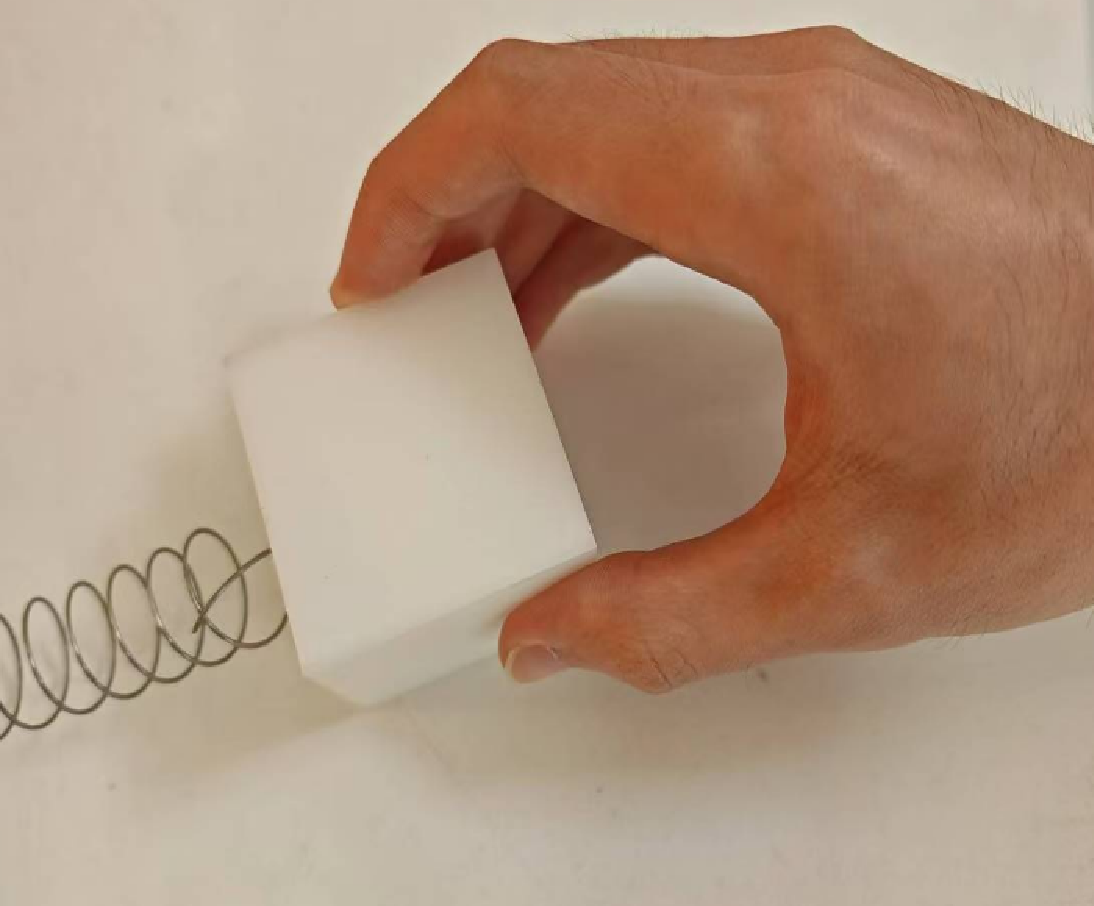
\includegraphics[width=\linewidth]{image/gesture-tracking-deviations-a.pdf}
    \caption{} % 子图标题 (a) 的内容
    \label{fig:gesture-tracking-deviations-a}
  \end{subfigure}
  \hfill % 水平填充间隔
  \begin{subfigure}{0.31\linewidth} % 子图 (b)
    \centering
    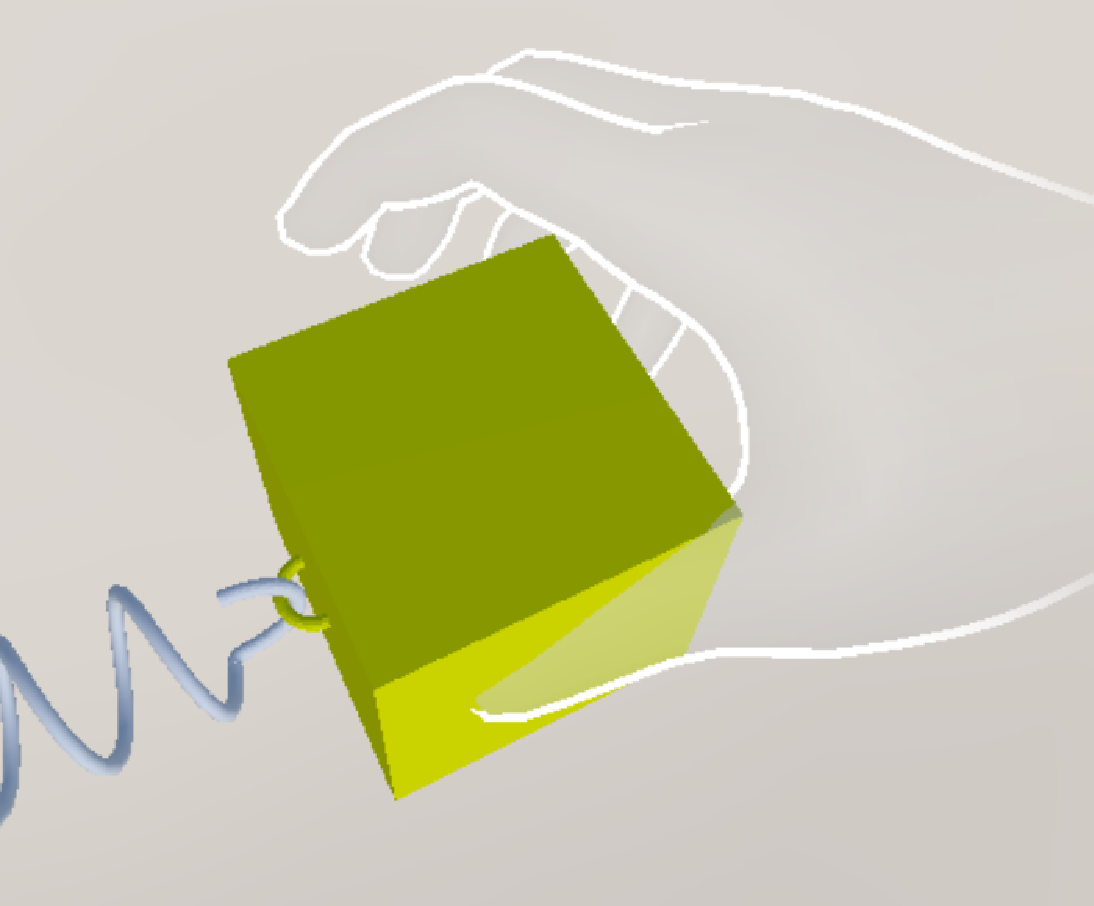
\includegraphics[width=\linewidth]{image/gesture-tracking-deviations-b.pdf}
    \caption{} % 子图标题 (b) 的内容
    \label{fig:gesture-tracking-deviations-b}
  \end{subfigure}
  \hfill % 水平填充间隔
  \begin{subfigure}{0.31\linewidth} % 子图 (c)
    \centering
    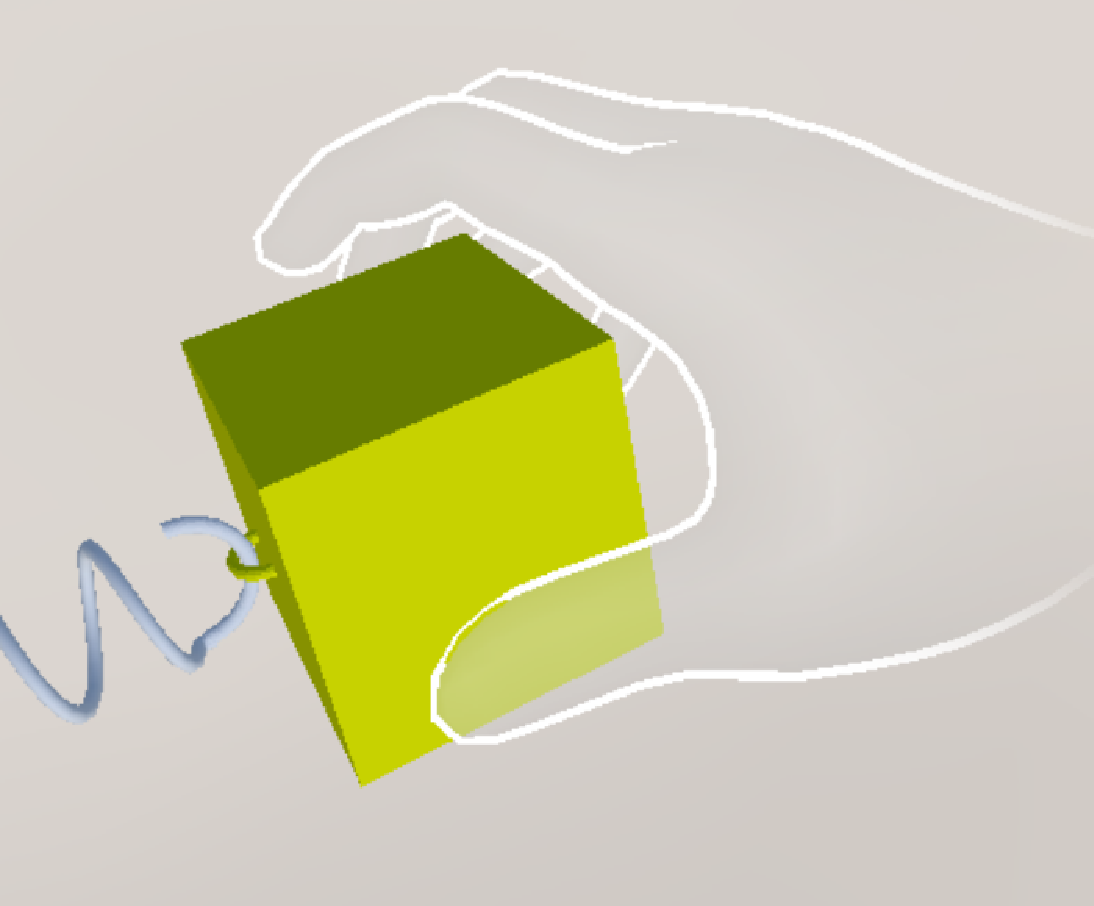
\includegraphics[width=\linewidth]{image/gesture-tracking-deviations-c.pdf}
    \caption{} % 子图标题 (c) 的内容
    \label{fig:gesture-tracking-deviations-c}
  \end{subfigure}
  \caption{Misalignment issue in gesture tracking. (\subref{fig:gesture-tracking-deviations-a}) Real interaction, (\subref{fig:gesture-tracking-deviations-b}) Virtual hand penetration, (\subref{fig:gesture-tracking-deviations-c}) Irregular object motion.}
  \label{fig:gesture-tracking-deviations}
\end{figure}


\paragraph{VIO Motion Independence}: The VIO's core motion (position, rotation) is solely driven by RIO sensor data. The VIO is assigned infinite mass within the physics engine, ensuring it remains unaffected by unintended virtual hand collisions, preventing unnatural jitter or displacement.

\paragraph{Gesture Parameterization \& Predefinition}: Hand gesture characteristics (joint positions, finger lengths, bending angles) are parameterized. For each VIO type, interaction-specific canonical gestures are predefined, optimized to match the VIO's geometry and intended manipulation method. Examples include a semi-closed grasp for cylindrical objects or an extended finger pose for button pressing.

\paragraph{Dynamic Collision Handling via Gesture Prediction}:
\begin{enumerate}
  \item Interaction Trigger Zone: A spherical bounding volume centered on the user's virtual palm defines the proximity region for potential interaction initiation (Fig. \ref{fig:bounding-volume}).
  \item Hand Collision Model: A simplified sphere tree model approximates the collision geometry of the virtual hand (e.g., spheres at key joints and palm) (Fig. \ref{fig:sphere-tree-model}).

  \begin{figure}
    \begin{subfigure}{0.48\linewidth} % 子图 (a)
      \centering
      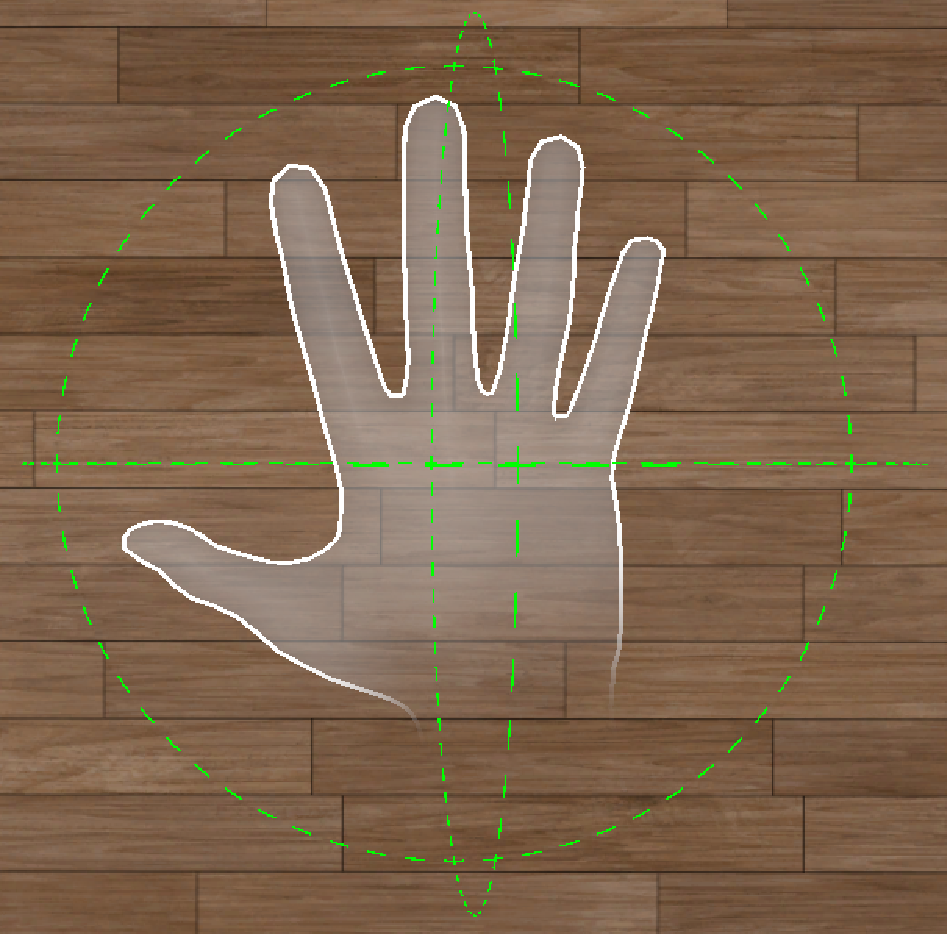
\includegraphics[width=\linewidth]{image/bounding-volume.pdf}
      \caption{} % 子图标题 (a) 的内容
      \label{fig:bounding-volume}
    \end{subfigure}
    \hfill % 水平填充间隔
    \begin{subfigure}{0.48\linewidth} % 子图 (b)
      \centering
      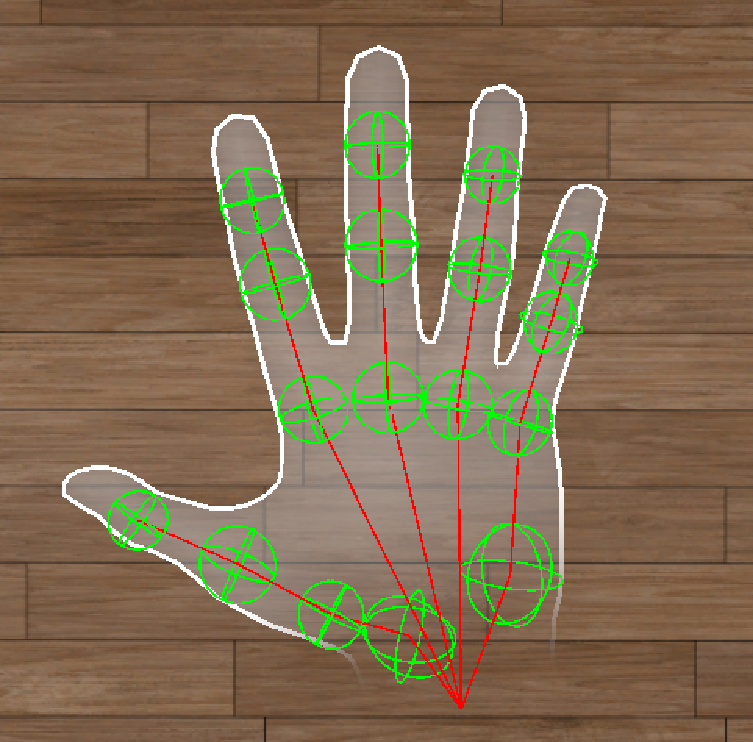
\includegraphics[width=\linewidth]{image/sphere-tree-model.pdf}
      \caption{} % 子图标题 (b) 的内容
      \label{fig:sphere-tree-model}
    \end{subfigure}
    \caption{Bounding volume and sphere tree model for the virtual hand. (\subref{fig:bounding-volume}) Spherical bounding volume, (\subref{fig:sphere-tree-model}) Sphere tree model.}
    \label{fig:bounding-volume-and-sphere-tree-model}
  \end{figure}

  \item State-Based Collision Strategy:
    \begin{enumerate}
      \item Interacting State: When the hand enters the trigger zone and the user's tracked gesture sufficiently matches the VIO's predefined interaction gesture, the system initiates the interaction: 
      \begin{enumerate}
        \item The virtual hand smoothly interpolates towards the predefined canonical pose to minimize visual penetration. \item Physics-based collision between the hand's sphere tree and the VIO is disabled to prevent penetration artifacts while the interaction gesture is active.
      \end{enumerate}

      \item Non-Interacting State: Outside the trigger zone or without a matching gesture: 
      \begin{enumerate}
        \item Physics-based collision using the hand's sphere tree is enabled. 
        \item This prevents the virtual hand from passing through the VIO. 
        \item Due to the VIO's infinite mass, collisions do not cause unrealistic VIO motion, only constraining the hand's position.
      \end{enumerate}
  \end{enumerate}

\end{enumerate}
\section{VRTI DESIGN}

\chadded[id=zheliku]{
  VRTI established closed-loop interactive systems for scenarios requiring synchronized tactile authenticity, operational safety, and visual extensibility. It can be applied to the following three types of interaction scenarios.
}

\begin{enumerate}
  \item \texttt{High-risk skill training domains} (e.g., industrial equipment maintenance, medical surgical procedures), where RIOs preserve proprioceptive motor chains (e.g., torque transmission, tissue puncture resistance) while VIOs overlay hazardous scenario visualization and operational guidance to mitigate hands-on risks.
  \item \texttt{Complex system cognition enhancement} (e.g., science experiment pedagogy, mechanical principle demonstration), leveraging RIOs to enable physically constrained interactions (e.g., spring oscillator dynamics, chemical reaction progression) while VIOs generate multidimensional dynamic data representations (e.g., force vector decomposition, molecular structure evolution) to establish multimodal cognitive closure.
  \item \texttt{Cross-space collaborative environments} (e.g., remote equipment servicing, distributed prototype design), utilizing RIOs to synchronize local operational parameters (e.g., tool torque, interface depression depth) while VIOs construct shared digital twins to enable collaborative decision-making through bidirectional haptic-visual feedback.
\end{enumerate}


\subsection{Experiment Scenario}
\chadded[id=zheliku]{
  In collaboration with Professor XXX % 提交版需匿名
  % Xiang Hua 
  and his team from the Physics Department of XXX
  % Beijing Normal 
  University, the experimental content was determined to be the verification of the law of conservation of momentum. We selected the experiment for the following reasons:
}
\begin{enumerate}
    \item It requires simultaneous perception of force (spring), time (trajectory), and system state (mass ratios).
    \item The phenomenon involves discontinuous state changes (collisions) challenging to simulate with static props.
    \item It demonstrates core physics principles transferable to other domains.
\end{enumerate}

The experimental setup consists of two blocks, A and B, connected by a spring. Students impart an initial velocity to block B by pulling it backward, causing the system to undergo periodic motion under the spring's influence. During the experiment, students observe visualized data on a panel to study the system's motion process, thereby verifying the law of conservation of momentum. The specific experiment scenario is illustrated in Figure \ref{fig:experiment-scenario}.

\begin{figure}
  \centering
  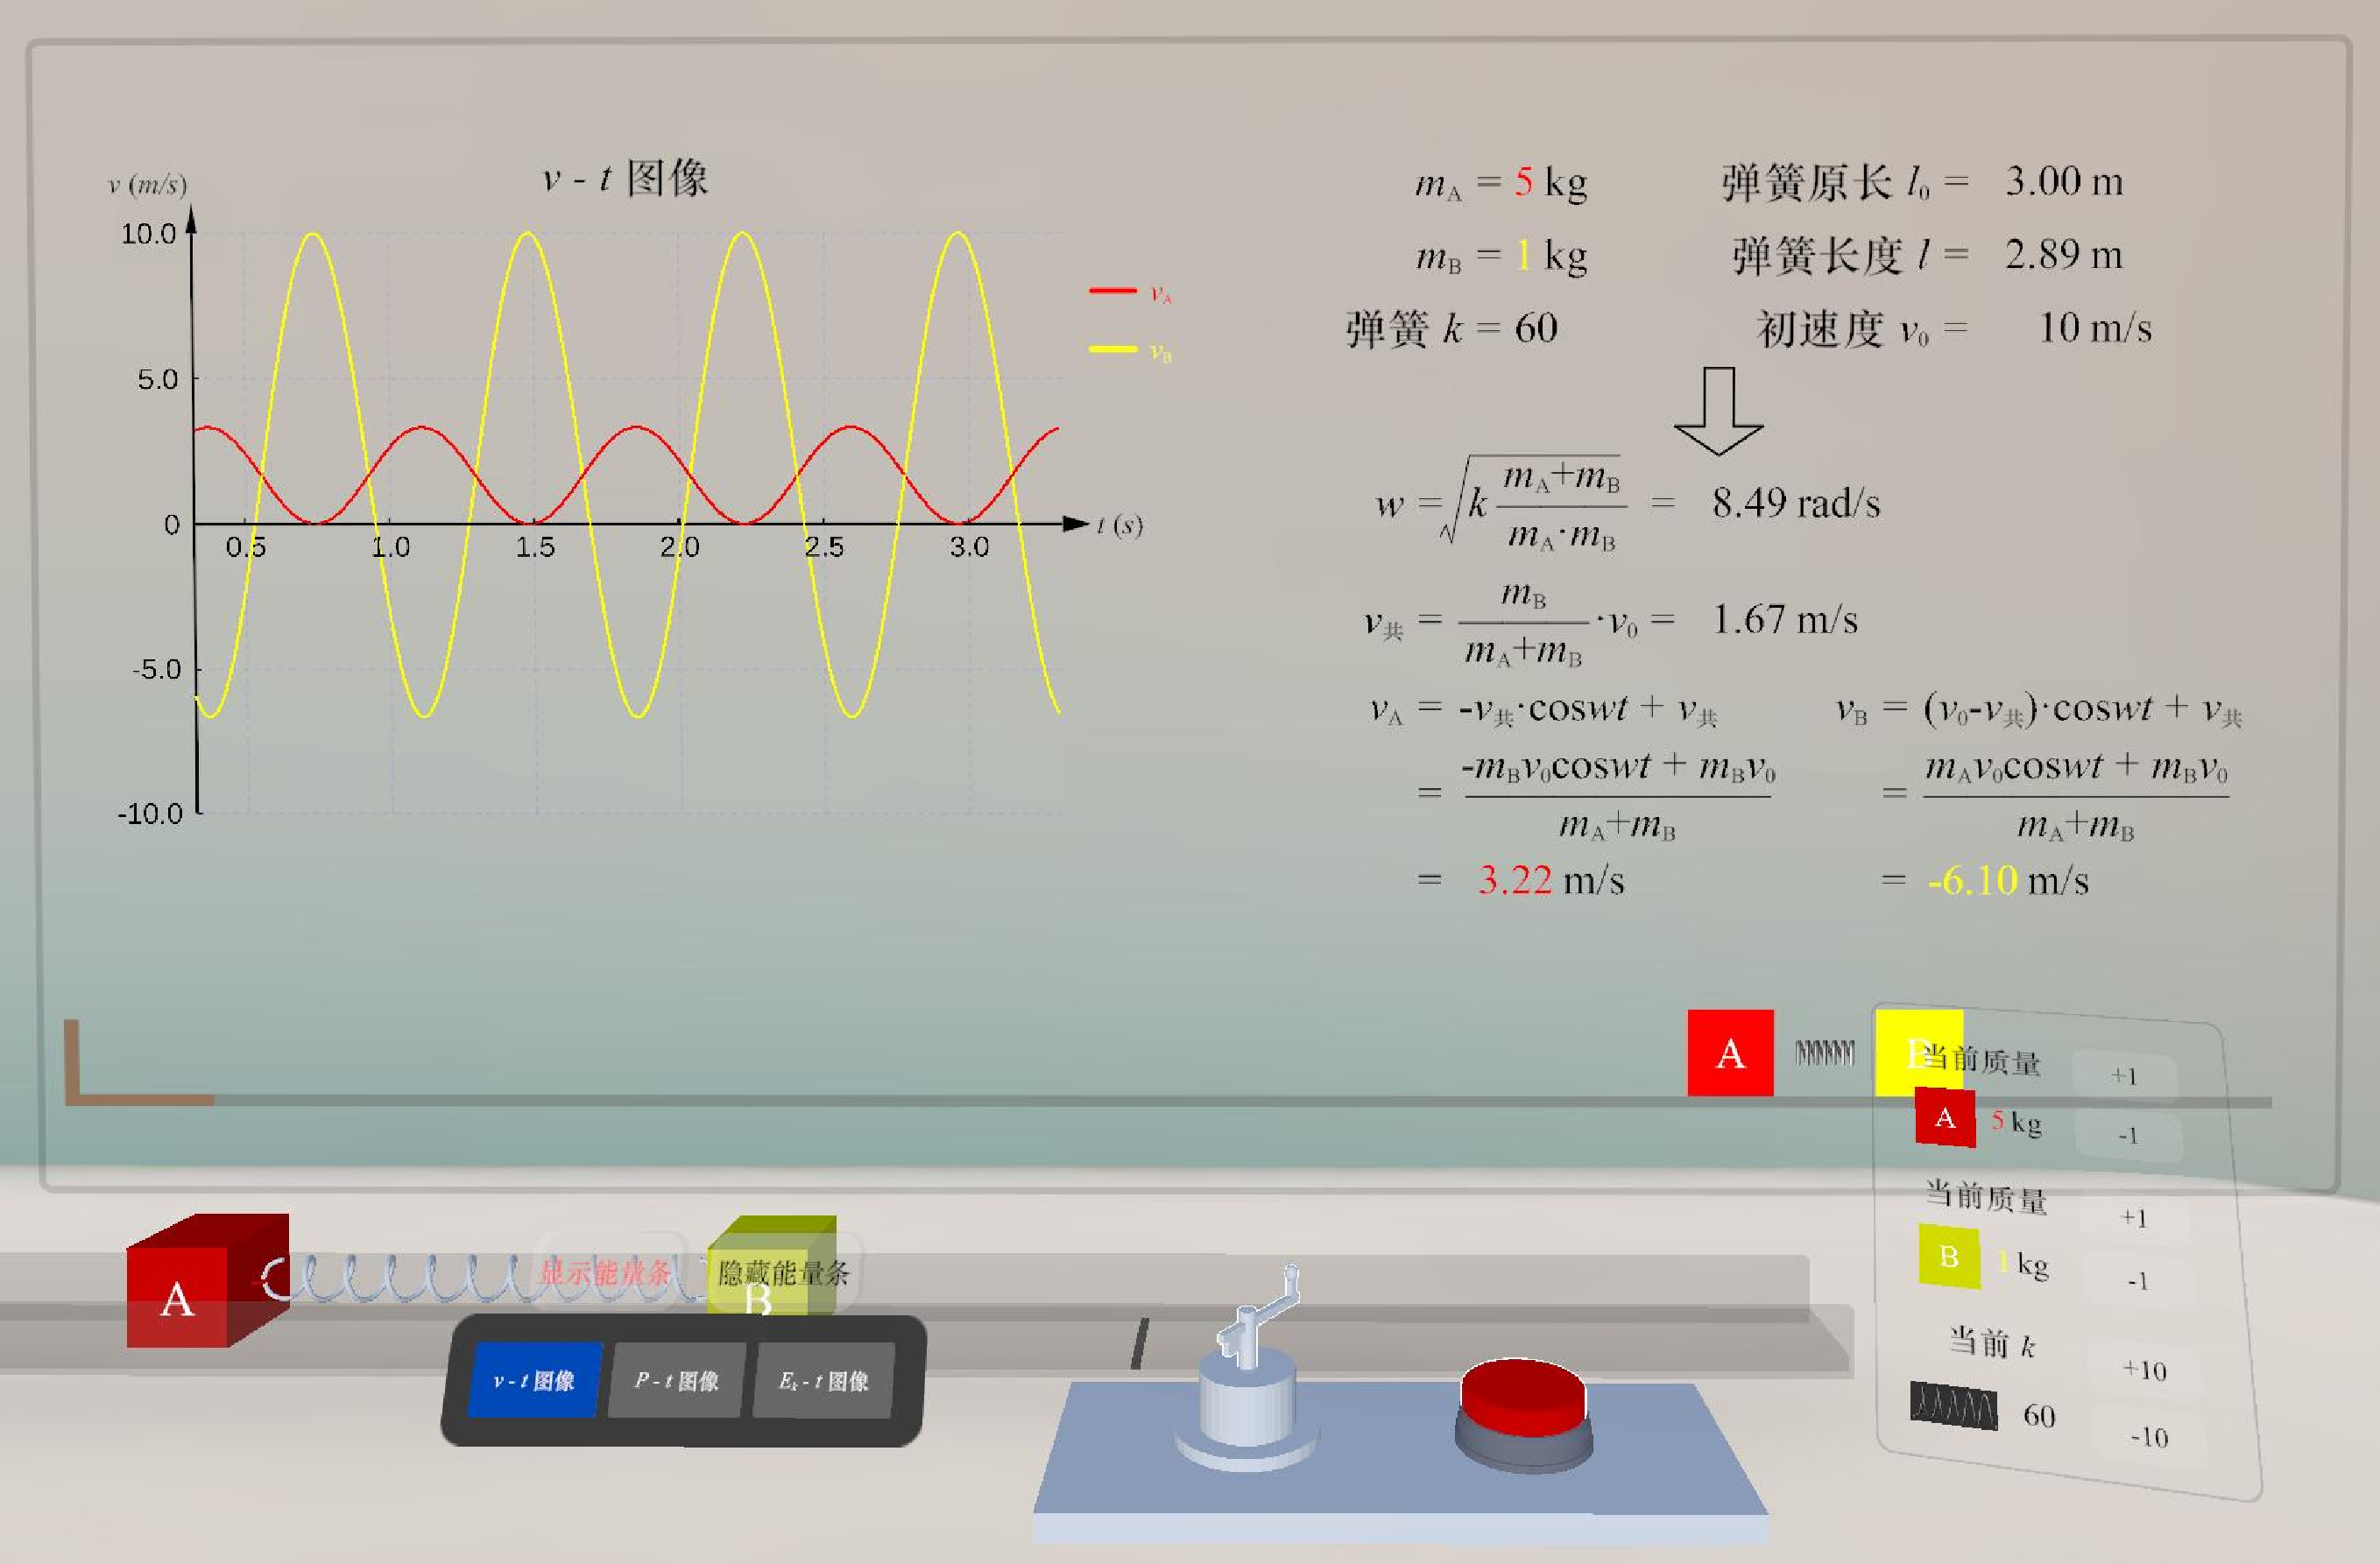
\includegraphics[width=\linewidth]{image/experiment-scenario.pdf}
  \caption{Momentum conservation experiment scenario.}
  \label{fig:experiment-scenario}
\end{figure}

Upon entering the experiment scenario, students first use their index finger to click a button on the parameter setting panel on the right to configure experimental parameters, including the masses of the two blocks and the spring constant. Next, they pull the block B to the right and release it when the force is appropriate, "launching" block B and observing the system's motion. Then, they rotate the knob to adjust the timeline of the motion process (clockwise for forward, counterclockwise for backward), exploring the characteristics of the visualized panel's graphs and the relationships between physical quantities. Finally, when the system reaches its final position, students press the button to reset the system and reconfigure the experimental parameters to continue their exploration.

On the left side of the visualization panel, three graphs: (1) $v$-$t$, (2) $P$-$t$, and (3) $E_k$-$t$ are provided to intuitively display the changes in corresponding physical quantities. The right side presents the calculation formulas for the corresponding physical quantities, showing their computational processes. Graph switching is implemented as button interactions to facilitate teaching needs during the experiment.

\subsection{Virtual-Real Twins}
Based on the experimental design for verifying the law of conservation of momentum, the implementation of VR twins includes a puller, a button, and a knob. Figure \ref{fig:structural-diagram} illustrates the structural design of each. The RIO and VIO for all three VR twins are derived from the same 3D model. The RIO is obtained through 3D printing, while the VIO is created by importing the model into Unity. Since the user's visual feedback is directly provided by the VIO, the VIO is rendered with color in the virtual environment, while the RIO remains uncolored.

\begin{figure*}[t]
  \centering
  \includegraphics[width=1\textwidth]{image/Structural-Diagram.pdf} % 使用\textwidth而非\linewidth
  \caption{Structural diagram of three VR twins.}
  \label{fig:structural-diagram}
\end{figure*}

\begin{figure*}[t]
  \centering
  \includegraphics[width=1\textwidth]{image/Interaction-Flow.pdf}
  \caption{Interaction flow of three VR twins.}
  \label{fig:interaction-flow}
\end{figure*}

\subsubsection{Puller}
The puller simulates pulling interactions and consists of a spring and a movable block. The left end of the spring is fixed, while the right end is connected to the block. Users pull the block to experience the spring's tension. A rail structure ensures the block moves along a straight path, preventing deviations during operation.

\subsubsection{Button}
The button is a common physical interaction device, allowing users to interact with the virtual environment by pressing it. It consists of a hollow cylindrical base and a slide switch, connected by a spring. When the button is pressed, the base remains stationary while the switch moves downward, compressing the spring. When released, the switch returns to its original position due to the spring's elasticity.

\subsubsection{Knob}
The knob simulates rotational interactions and comprises a base and a rotatable handle. Users rotate the handle to operate the knob. The rotational axis providing realistic rotational feedback to simulate resistance and restoring force at different angles.

\subsection{Interaction Design}
Among the three VR twins, the puller simulates pulling interactions, such as elastic rods or springs, providing tension proportional to the pulling distance. The button simulates touch and press interactions, such as keyboard keys or button triggers, providing elastic force proportional to the pressing distance. The knob simulates rotational interactions, such as dials or steering wheels, without providing significant feedback force. Figure \ref{fig:interaction-flow} illustrates the interaction flow of the three VR twins.

Due to the relatively large size of the block, the puller is designed for grasping interactions. User grasps the block, pulls the spring backward to a certain distance to trigger the puller, and then releases the block to allow the spring to rebound, completing the interaction. The button is designed for pressing interactions. User places their hand above the switch, presses it to a certain distance to activate the button, and then lifts their hand to complete the interaction. Due to the relatively small size of the handle, the knob is designed for pinching interactions. User pinches the head of the handle with their fingers, rotates it around the central axis to adjust its angle, and releases their fingers to complete the interaction. During the interaction, the button only records whether it is pressed, while the puller records both whether it is pulled and the magnitude of the force applied.
\section{EXPERIMENT AND EVALUATION}
The experiment utilized the Meta Quest 3 as the VR headset to provide users with visual information, while VR twins served as the interaction method to deliver haptic feedback. The program's interaction logic and visualization scenarios were implemented using Unity 2021.3.32f1c1. The VR twins employed gesture-tracking technology to visualize the user's physical hand as a virtual hand for interaction, with real-time data updates and synchronization achieved through sensing technology. Gesture tracking was implemented using the Meta XR All-in-One SDK (v63). The system framework is illustrated in Figure \ref{fig:system-framework-flowchart}.

\begin{figure*}[t]
  \centering
  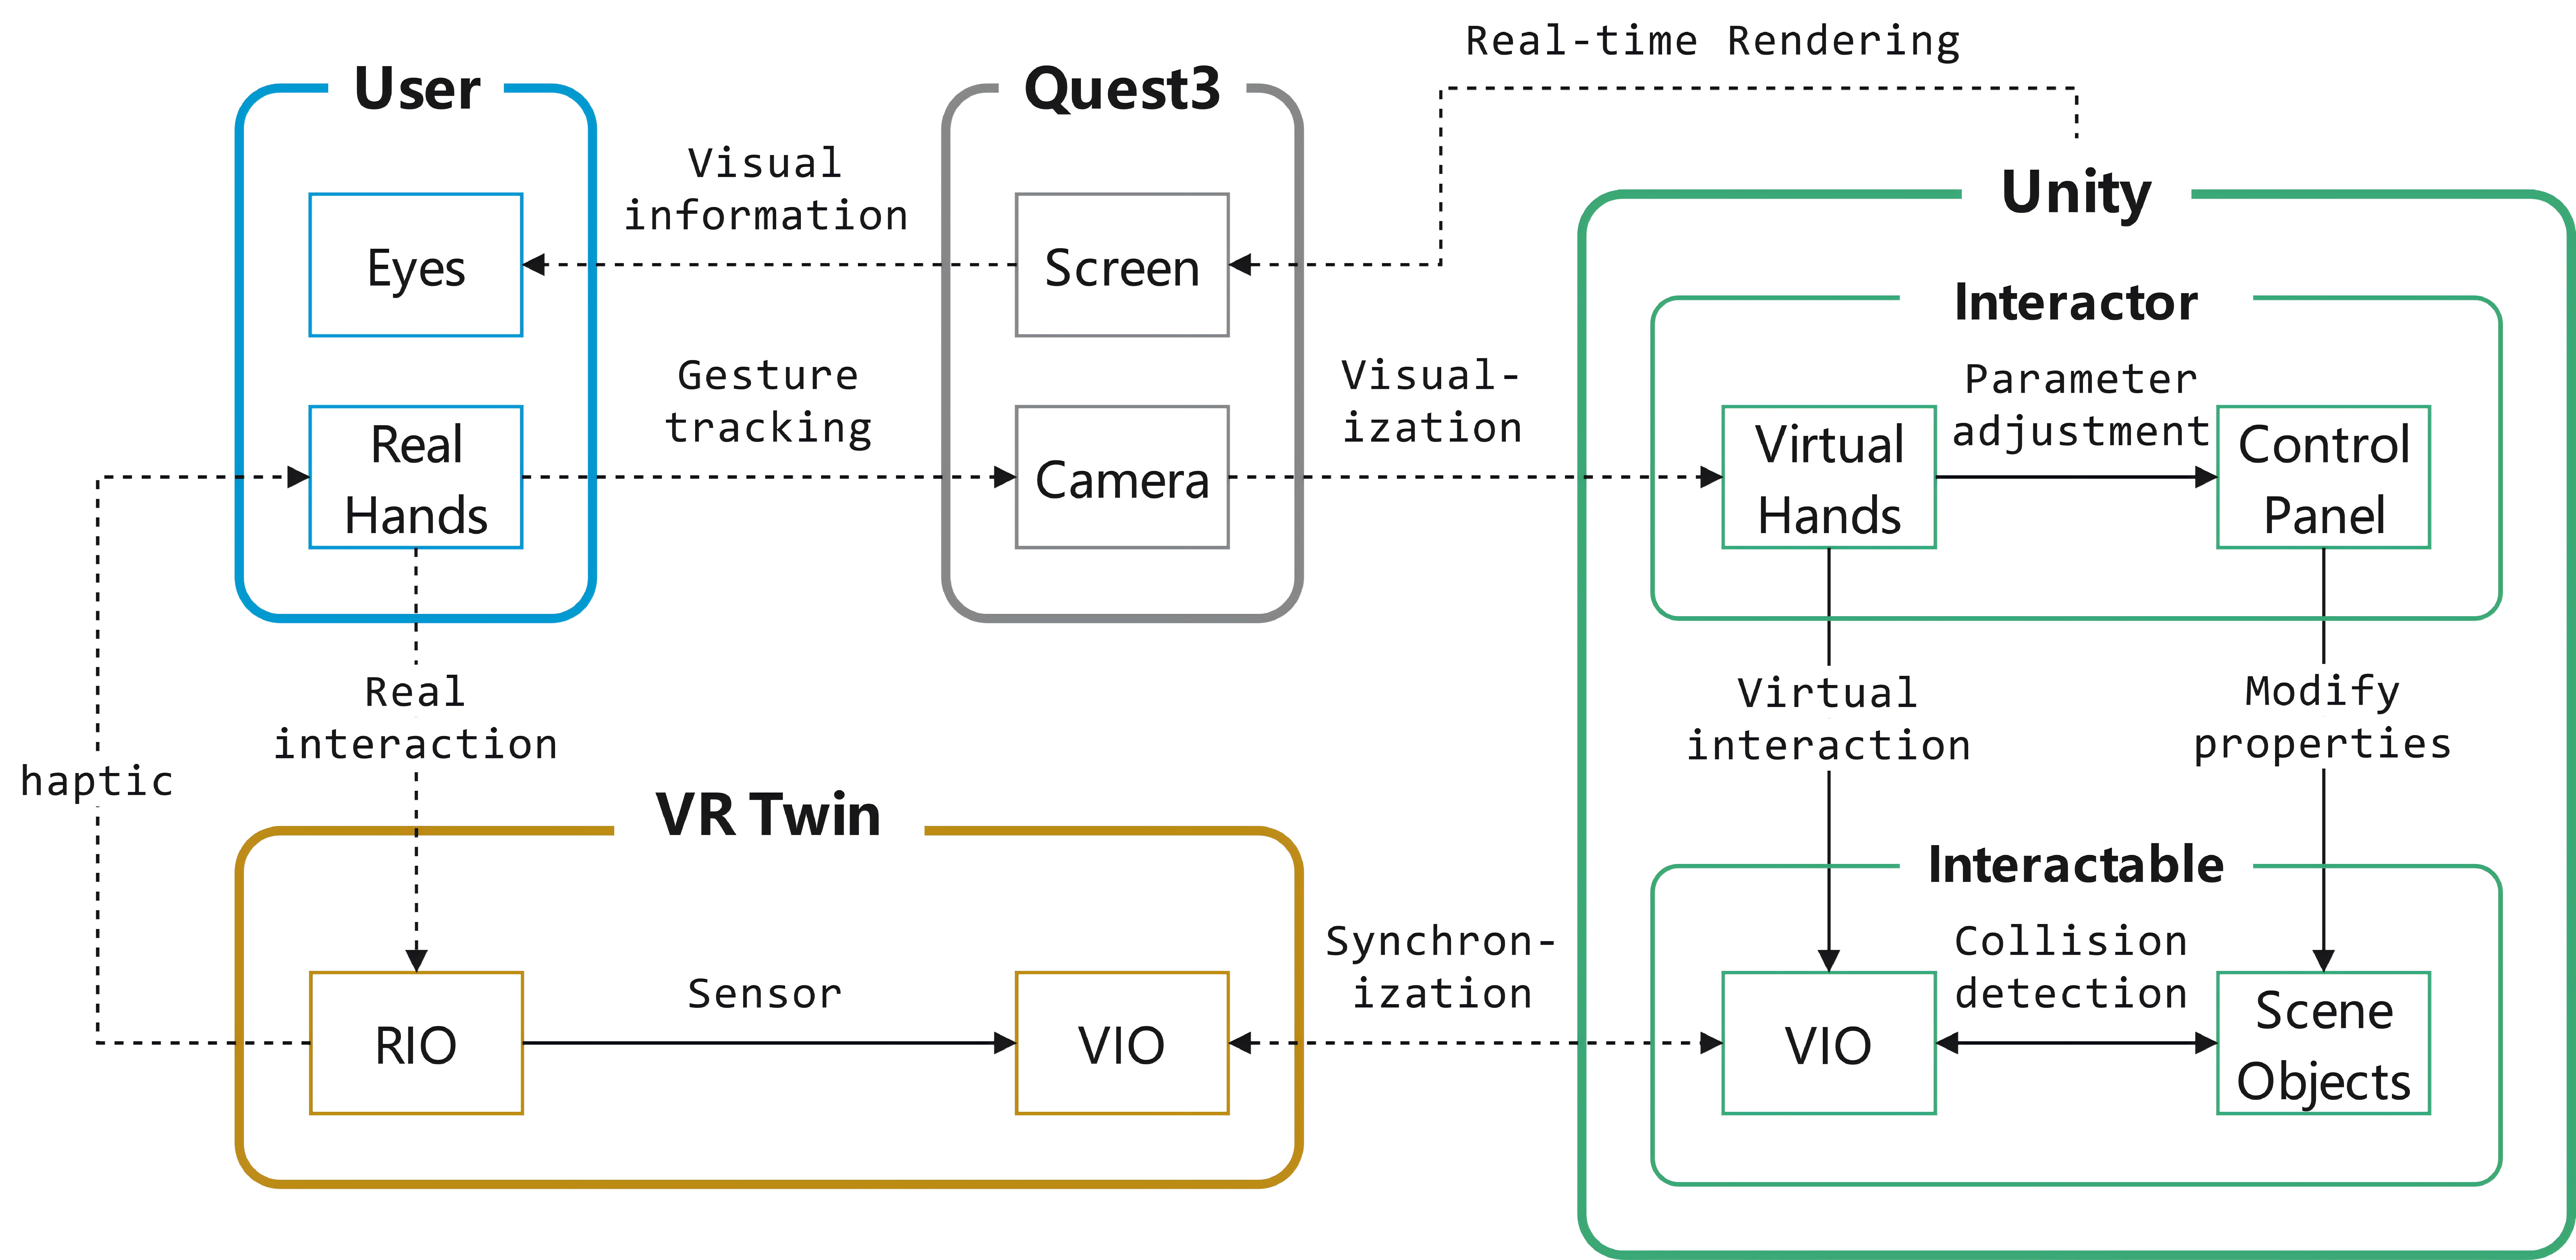
\includegraphics[width=1\textwidth]{image/system-framework-flowchart.pdf}
  \caption{System framework flowchart.}
  \label{fig:system-framework-flowchart}
\end{figure*}

\subsection{Evaluation Methods}
This study compares VRTI (with realistic haptic feedback, experimental group) and GI (without realistic haptic feedback, control group). The only difference between the two interaction methods is the presence or absence of real haptic feedback. Through a comparative experiment, the study investigates the impact of real haptic feedback on students' physics experiments in terms of cognitive load, learning motivation, immersion, and learning outcomes.

\subsubsection{User Experience}
\begin{enumerate}
  \item {\texttt{Cognitive Load}}: Cognitive load is measured using the Klepsch Scale \cite{klepsch2017development}, which assesses three dimensions: intrinsic cognitive load, extraneous cognitive load, and germane cognitive load. In haptic feedback tasks, multimodal interactions between haptic and visual/auditory information may reduce extraneous cognitive load through "attention guidance" but could also increase germane cognitive load due to "cross-modal switching."

  \item {\texttt{Learning Motivation}}: Learning motivation is measured using the Keller Scale \cite{keller1983motivational}, based on the ARCS model of motivation. It evaluates four dimensions: Attention, Relevance, Confidence, and Satisfaction, assessing learners' internal drive to engage in and complete learning tasks. When exposed to new technologies like haptic feedback, learners' intrinsic motivation (e.g., curiosity and desire to explore) or extrinsic motivation (e.g., rewards for task completion) may significantly influence their engagement and learning effectiveness. Higher motivation increases the likelihood of students persisting through challenges, thereby leveraging haptic feedback technology for effective learning.

  \item {\texttt{Immersion}}: Immersion is measured using the Schubert Scale \cite{schubert2001experience}, focusing on the sense of presence in the virtual environment. It comprehensively evaluates students' immersion and sense of control through three dimensions: spatial presence, involvement, and perceived realism of the virtual environment.
\end{enumerate}

All scales were translated and localized to ensure their suitability for the cultural and educational context of this experiment.

\subsubsection{Physics Knowledge}
The physics knowledge test was provided by Professor XXX
% Xiang Hua 
and his team from the Physics Department of XXX
% Beijing Normal 
University. It consists of a pre-test and a post-test.

\begin{enumerate}
  \item {\texttt{Pre-test}}: Includes 16 items, with 6 focusing on basic physics knowledge to assess students' foundational understanding and 10 related to the experiment for comparison with the post-test results.

  \item {\texttt{Post-test}}: Includes 16 items, with 10 being similar to the pre-test's experiment-related questions (with changes in narrative and data) and 6 being more challenging comprehensive application questions to evaluate students' critical thinking and ability to synthesize knowledge.
\end{enumerate}

Both tests include an "I don't know" option to reduce guessing tendencies and obtain more accurate assessment data.

\subsubsection{Semi-Structured Interviews}
After the user experiment, semi-structured interviews were conducted to explore participants' experiences with VRTI and immersive learning, with follow-up questions to delve deeper. Examples include:

\begin{enumerate}
  \item "What is your overall impression of VRTI?"
  
  \item "What do you think are the differences between VRTI and GI?"
  
  \item "You mentioned 'immersion.' Could you provide an example?"
\end{enumerate}

The interviews aimed to capture personalized perspectives and in-depth insights while ensuring data completeness. Face-to-face interviews were conducted in a private, distraction-free environment, with recordings and notes taken after obtaining participants' consent.

\subsection{Evaluation Process}
\subsubsection{Participants}
A total of 64 high school sophomores from XXX
% Beijing Jingshan 
School were recruited for the experiment. All participants had previously studied the relevant foundational physics knowledge in class. The students were randomly and evenly divided into two groups:

\begin{enumerate}
  \item Experimental Group (N=32): used VRTI.

  \item Control Group (N=32): used GI.
\end{enumerate}

\subsubsection{Experimental Procedure}
To ensure the validity of the results, all participants received a unified experimental introduction and operational guidance before starting the experiment (Figure \ref{fig:experimental-procedure}). The procedure consisted of the following four steps:

\begin{enumerate}
\item {\texttt{Pre-test}}: Students independently completed a pre-test questionnaire, which took approximately 10 minutes.

\item {\texttt{Experimental Introduction}}: Students watched an instructional video to familiarize themselves with the experimental operations and procedures, which took approximately 5 minutes.

\item {\texttt{Experimental Operation}}: Students performed the experiment according to their assigned group, which took approximately 15 minutes.

\item {\texttt{Post-test}}: Students independently completed a post-test questionnaire, which included 30 user experience evaluation items (cognitive load, learning motivation, immersion) and 15 physics knowledge evaluation items, taking approximately 30 minutes.

\begin{figure}
  \begin{subfigure}{0.48\linewidth} % 子图 (a)
    \centering
    \includegraphics[width=\linewidth]{image/experimental-introduction.pdf}
    \caption{} % 子图标题 (a) 的内容
    \label{fig:experimental-introduction}
  \end{subfigure}
  \hfill % 水平填充间隔
  \begin{subfigure}{0.48\linewidth} % 子图 (b)
    \centering
    \includegraphics[width=\linewidth]{image/experimental-operation.pdf}
    \caption{} % 子图标题 (b) 的内容
    \label{fig:experimental-operation}
  \end{subfigure}
  \caption{Experimental procedure demonstration. (\subref{fig:experimental-introduction}) Experimental introduction, (\subref{fig:experimental-operation}) Experimental operation.}
  \label{fig:experimental-procedure}
\end{figure}

\end{enumerate}

Throughout the experiment, group assignments were randomized to ensure balance between the groups. Teaching assistants supervised the entire process to ensure that each participant strictly followed the experimental procedure.

\subsection{Results Analysis}
\begin{figure*}[t]
  \centering
  \begin{subfigure}{0.45\textwidth} % 子图 (a)
    \centering
    \includegraphics[width=\linewidth]{image/pre-test-result.pdf}
    \caption{} % 子图标题 (a) 的内容
    \label{fig:pre-test-result}
  \end{subfigure}
  \hspace{0.05\textwidth} % 水平填充间隔
  \begin{subfigure}{0.45\textwidth} % 子图 (b)
    \centering
    \includegraphics[width=\linewidth]{image/user-experience-result.pdf}
    \caption{} % 子图标题 (b) 的内容
    \label{fig:user-experience-result}
  \end{subfigure}
  \caption{Pre-test and user experience results. (\subref{fig:pre-test-result}) Pre-test result, (\subref{fig:user-experience-result}) User Experience result.}
  \label{fig:pre-test-and-user-experience-result}
\end{figure*}

\begin{figure*}[t]
  \centering
  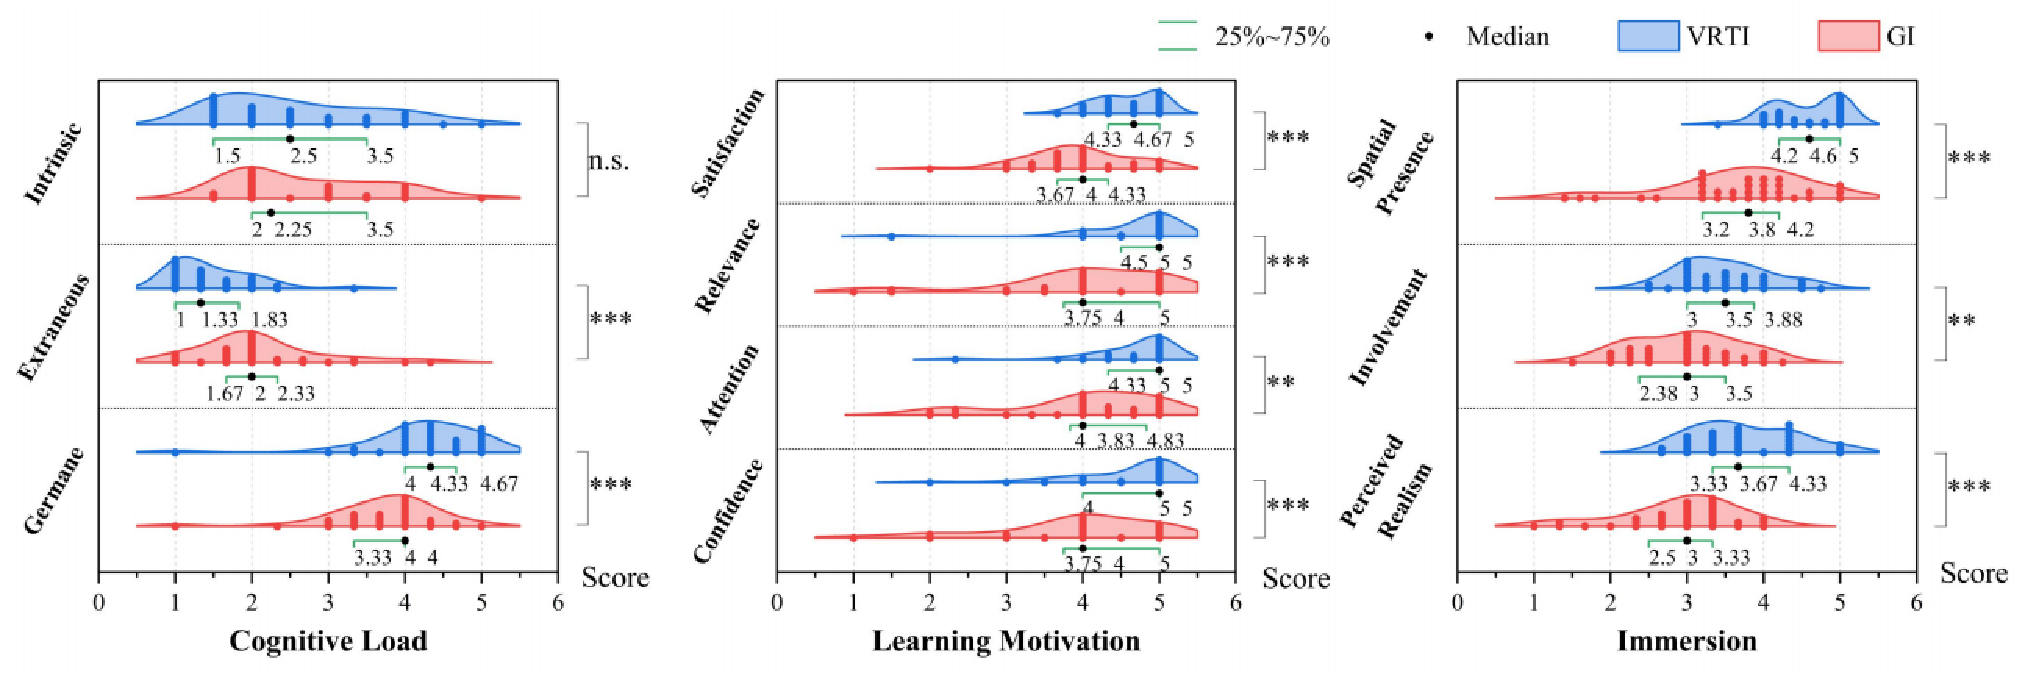
\includegraphics[width=\textwidth]{image/three-user-experience-result.pdf} % 使用\textwidth而非\linewidth
  \caption{Comparison of each user experience between VRTI and GI.}
  \label{fig:three-user-experience-result}
\end{figure*}

According to Shapiro-Wilks tests, only the experiment-related content test results in the experimental group followed a normal distribution, while all other measures violated this assumption. Consequently, the Mann-Whitney U test was employed to analyze between-group differences. Significance levels were denoted as follows: $p \le 0.05$ (*) for significant differences, $p \le 0.01$ (**) for highly significant differences, and $p \le 0.001$ (***) for extremely significant differences. Effect sizes were interpreted as: $|r| \le 0.1$ indicating small effects, $0.1 < |r| \le  0.3$ representing medium effects, and $d > 0.5$ reflecting large effects.

\subsubsection{Prior Analysis}
The pre-test included 6 basic physics concept questions and 10 experiment-related questions, each scored 1 point, totaling 16 points. Figure \ref{fig:pre-test-result} shows the pre-test results for both groups, with bar lengths representing the mean (Mean) and black error bars indicating 1.0 × standard deviation (SD). The Mann-Whitney U Test (M-U Test) results revealed no significant differences between the experimental and control groups in basic physics concepts ($p=0.600$), momentum conservation knowledge ($p=0.984$), or overall scores ($p=0.834$). Therefore, it can be concluded that the two groups had comparable prior physics knowledge.

Figure \ref{fig:user-experience-result} compares the user experience between the experimental and control groups across three dimensions: cognitive load, learning motivation, and immersion.Solid circles above each group represent sample points, with kernel smoothing used to fit curves describing their distribution. Below, Type I boxplots show the 25\% (Q1), 50\% (Q2), and 75\% (Q3) quartiles.

\subsubsection{Cognitive Load}
There was no significant difference in intrinsic cognitive load between the two groups ($Z=-0.720, p=0.472, |r|=0.127$). The extraneous cognitive load in the experimental group was significantly lower than that in the control group ($Z=-3.538, p<0.001, |r|=0.625$), showing a large effect. Conversely, the germane cognitive load in the experimental group was significantly higher ($Z=-3.337, p=0.001, |r|=0.590$), also with a large effect. These results can be explained as follows:

\begin{enumerate}
\item {\texttt{Intrinsic Cognitive Load}}: The addition of realistic haptic feedback does not affect the inherent complexity of the learning task, which aligns with Cognitive Load Theory. Intrinsic cognitive load is related to the essential complexity of the task and is difficult to change significantly through interaction methods.

\item {\texttt{Extraneous Cognitive Load}}: VRTI reduces unnecessary load caused by redundant or distracting information during operations by providing realistic haptic feedback.

\item {\texttt{Germane Cognitive Load}}: Realistic haptic feedback promotes the construction and automation of cognitive structures, enhancing learning and understanding.
\end{enumerate}

\subsubsection{Learning Motivation}
The experimental group showed significant improvements in attention ($Z=-3.382, p=0.001, |r|=0.598$), relevance ($Z=-3.313, p=0.001, |r|=0.586$), confidence ($Z=-3.001, p=0.003, |r|=0.531$), and satisfaction ($Z=-4.127, p<0.001, |r|=0.730$), all with large effects. These results can be explained as follows:

\begin{enumerate}
  \item {\texttt{Attention}}: Realistic haptic feedback in immersive learning environments attracts learners' interest more effectively.

  \item {\texttt{Relevance}}: Customized content design enhances the connection between the learning material and the learners.

  \item {\texttt{Confidence}}: Immediate feedback and interactive experiences provided by VRTI boost learners' confidence.

  \item {\texttt{Satisfaction}}: Realistic haptic feedback provides a sense of achievement during interactions, increasing learners' satisfaction.
\end{enumerate}

\subsubsection{Immersion}
The experimental group showed significant improvements in spatial presence ($Z=-4.524, p<0.001, |r|=0.800$), involvement ($Z=-2.774, p=0.006, |r|=0.490$), and perceived realism ($Z=-4.102, p<0.001, |r|=0.725$), all with large effects. These results can be explained as follows:

\begin{enumerate}
  \item {\texttt{Spatial Presence}}: Realistic haptic feedback significantly enhances learners' sense of spatial presence.

  \item {\texttt{Involvement}}: The well-designed interaction of VR twins significantly increases learners' engagement.

  \item {\texttt{Perceived Realism}}: High-fidelity visual and haptic experiences in VRTI significantly enhance the realism of the learning environment.
\end{enumerate}

\subsubsection{Learning Outcomes}
Figure \ref{fig:improvements-result} presents the comparative results of pre-test and post-test improvements in momentum concept, experimental understanding, and total scores, along with performance on comprehensive application. Both momentum concept and experimental comprehension assessments consisted of 5 test items each, with each item worth 1 point (total 10 points).

The experimental group showed significant improvement in experimental understanding ($Z=-1.967, p=0.05, |r|=0.347$), with a medium effect, but no significant improvement in momentum concept ($Z=-0.354, p=0.724, |r|=0.063$) or overall scores ($Z=-1.714, p=0.087, |r|=0.303$). Additionally, the experimental group performed significantly better in comprehensive application tests ($Z=-2.828, p=0.005, |r|=0.500$), with a large effect. This indicates that VRTI, through realistic haptic feedback, helps learners understand experimental content more intuitively and enhances their comprehensive application abilities. However, mastery of momentum concepts relies more on learners' prior knowledge and abstract thinking skills, which VRTI has limited impact on.

\begin{figure}
  \centering
  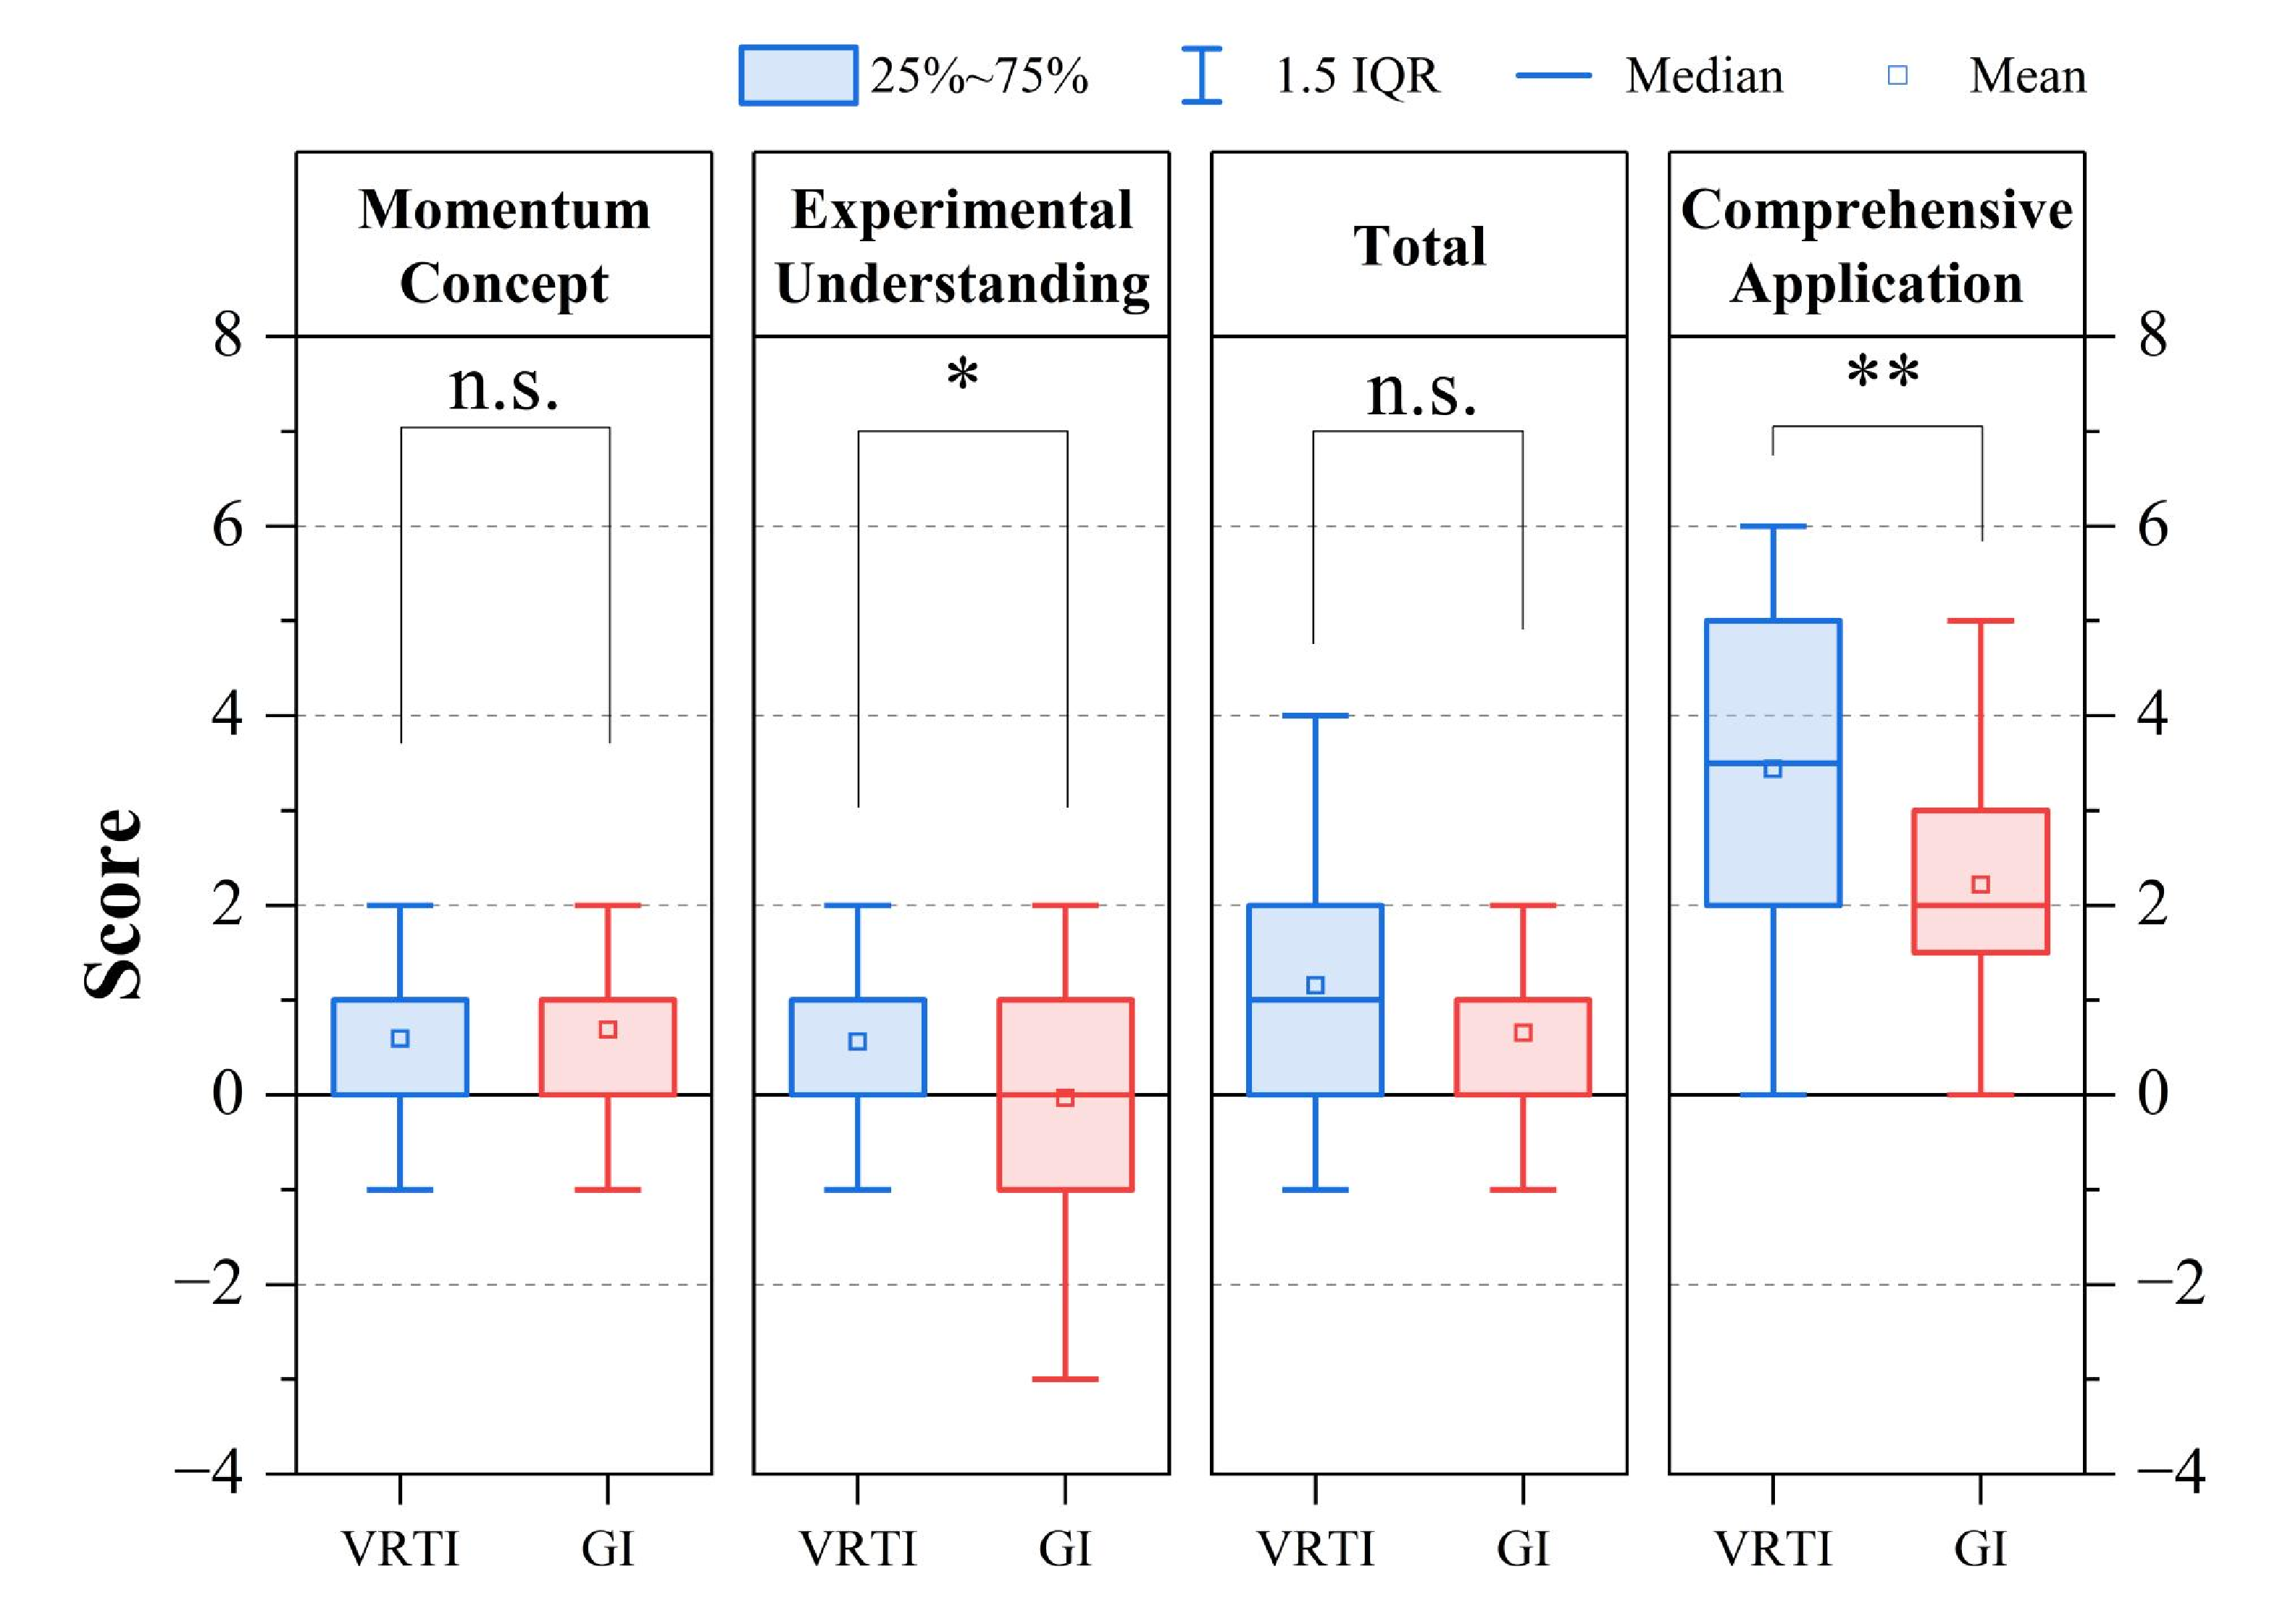
\includegraphics[width=0.8\linewidth]{image/improvements-result.pdf}
  \caption{The comparative results of pre-test and post-test improvements in momentum concept, experimental understanding, and total scores, along with performance on comprehensive application.}
  \label{fig:improvements-result}
\end{figure}

\subsubsection{Interview Results}
After the experiment, semi-structured interviews were conducted with participants to explore their subjective experiences with VRTI and GI. Key findings include:

\begin{enumerate}
  \item {\texttt{Overall Experience}}: Most users gave positive feedback on the haptic feedback, with one user stating, "VRTI allowed me to feel the weight and resistance of objects, making the operation more immersive." However, some users mentioned that prolonged use of GI could lead to arm fatigue: "Keeping my arms suspended for a long time during GI made me feel tired."

  \item {\texttt{Comparison with GI}}: Users generally agreed that the VRTI outperformed GI in terms of haptic feedback and operational intuitiveness. One user noted, "GI offers freedom of movement, but the lack of realistic haptic feedback makes it feel incomplete." Conversely, some users highlighted the flexibility of GI: "GI allows me to adjust hand positions freely, while the VRTI requires fixed positions."

  \item {\texttt{Immersion Experience}}: Users widely acknowledged that the VRTI significantly enhanced their sense of immersion in the virtual environment. One user explained, "When I pulled the spring, I could feel its resistance, which made me feel like I was actually conducting a physical experiment." However, some users reported that the quality of haptic feedback degraded with frequent use: "After multiple experiments, the haptic feedback of the device became less responsive."

  \item {\texttt{Improvement Suggestions}}: Users proposed several suggestions for improving the VRTI. For instance, one user recommended optimizing the support structure of the device to reduce operational fatigue: "If a support frame could be designed to keep the arms from being suspended all the time, the operation would be more comfortable." Additionally, users emphasized the need to enhance the durability of the device: "The haptic feedback of the device diminished after repeated use, and I hope this can be improved in the future."
\end{enumerate}
\section{LIMITATIONS AND FUTURE WORK}
Currently, the deployment of RIO and VIO in the VR twin system remains semi-automated, requiring manual adjustments to ensure precise alignment. During the course of this study, limitations in the VR headset's functionality made it difficult to capture camera images for automatic positioning. Relying solely on sensor technology for precise positioning is costly and may introduce additional base station deployments, thereby increasing system complexity. Future research will explore fully automated deployment methods, enabling precise RIO positioning and real-time VIO reconstruction as soon as the user dons the VR headset. By integrating advanced computer vision techniques with machine learning algorithms, dynamic prediction and adjustment of alignment errors will be achieved, facilitating spatial alignment without human intervention.

Another limitation is that current system supports only single-user interaction, whereas multi-user scenario (e.g., group experiments or team problem-solving activities) require synchronized interaction and shared virtual environments. Future research will investigate the extension of multi-user interaction, focusing on the development of shared virtual environments that support collaborative activities. Additionally, the potential educational value of VRTI will be explored, particularly in the context of collaborative learning modes in VR.

In addition, user feedback has highlighted issues with the durability of haptic feedback devices and the physical fatigue associated with prolonged interaction, which may impact the system's long-term usability and user satisfaction. Future research will prioritize enhancing the durability of interaction devices. Advanced materials will be employed to improve the lifespan and responsiveness of haptic feedback devices. Concurrently, ergonomic design principles will be incorporated to reduce user interaction burden.

Finally, current system's experimental setup and user interaction rely on predefined rules, limiting its adaptability to diverse learning scenario and personalized learning needs. Future research will focus on integrating AI into the VRTI to analyze user's behavior, predict learning requirements, and dynamically adjust the experimental environment. For instance, AI could guide users through complex experiments, provide personalized feedback, and recommend additional learning resources based on progress. Furthermore, AI-driven data analysis could be employed to assess learning outcomes and inform improvements to both the system and the curriculum.
\section{CONCLUSION}
This paper addresses the lack of haptic feedback in Gesture Interaction (GI) within VR immersive learning environments by proposing a Virtual-Real Twin Interaction (VRTI). For the momentum conservation experiment in physics learning at high school, three types of Virtual-Real twin (VR twin) were designed and implemented, supporting grasping, pressing, and pinching hand manipulations. Comparative evaluations between VRTI and GI in the momentum conservation experiment scenario demonstrate that the former significantly enhances user learning motivation and immersion without significantly increasing cognitive load. Moreover, it better aids users in understanding experimental content and improves their ability to apply knowledge comprehensively. Future research will explore the application of VR twins in other physics learning scenarios, improve hardware structures, and optimize interaction methods to enhance user learning experiences and operational comfort.

\begin{credits}
\subsubsection{\ackname} 
This study was supported by the Natural Science Foundation of China (No.62377004).

\subsubsection{\discintname}
The authors declare no competing interests.
\end{credits}


\bibliography{VRTI-bib}

\end{document}